% \chapter{Estado del Arte}\label{chapter:state-of-the-art}

% El presente capítulo tiene como objetivo analizar los fundamentos teóricos, tecnológicos y los sistemas existentes relacionados con la farmacovigilancia digital y el desarrollo de plataformas de autorreporte clínico. 
% Se aborda el estudio de soluciones implementadas a nivel internacional, así como las tecnologías y estándares utilizados en sistemas de salud digital, con el propósito de establecer una base sólida que sustente el diseño e implementación del sistema propuesto.
% Asimismo, se revisan conceptos relacionados con el modelado de datos clínicos y estándares de interoperabilidad que garantizan la consistencia y calidad de la información.

% \section{Análisis de sistemas de autorreporte clínico existentes}
% % Análisis de VAERS, V-Safe, etc.

% En el contexto de la farmacovigilancia moderna, diversos sistemas han sido desarrollados con el objetivo de facilitar la notificación de eventos adversos posteriores a la vacunación. 
% Estos sistemas difieren en su enfoque, arquitectura y nivel de digitalización, lo que impacta directamente en la calidad y disponibilidad de la información recolectada.
% A continuación, se analizan algunas de las principales soluciones implementadas a nivel internacional.

% \subsection{Vaccine Adverse Event Reporting System (VAERS)}

% % Descripción general
% % Tipo de vigilancia (pasiva)
% % Actores que reportan
% % Canal de notificación (web principalmente)
% % Fortalezas del sistema
% % Limitaciones

% \begin{figure}[htbp]
%     \centering
%     
\includegraphics[scale=0.5]{Graphics/vaers-logo.png}
%     \caption{Logotipo del sistema VAERS (vaers.hhs.gov)}
%     \label{fig:figura1}
% \end{figure}

% % Descripción general
% El \textit{Vaccine Adverse Event Reporting System} (VAERS) \cite{vaers_official} es un sistema nacional de vigilancia de seguridad de vacunas en los Estados Unidos, diseñado para el monitoreo de eventos adversos posteriores a la inmunización \cite{cdc_vaers}. 
% Este sistema se enmarca en el proceso de supervisión de vacunas tras su aprobación por la \textit{Food and Drug Administration} (FDA) \cite{fda_vaers}, y
% es administrado conjuntamente por la FDA y los \textit{Centers for Disease Control and Prevention} (CDC) \cite{cdc_vaers,fda_vaers}, y funciona como un repositorio centralizado para la recolección y análisis de reportes de eventos adversos asociados a la vacunación.

% % Tipo de vigilancia
% VAERS se clasifica como un sistema de vigilancia pasiva, ya que depende de la notificación voluntaria de eventos adversos por parte de los usuarios, en lugar de la recolección activa de datos por parte de las instituciones de salud \cite{cdc_vaers}. 
% Este enfoque permite una amplia cobertura poblacional, aunque introduce limitaciones asociadas a la calidad y completitud de los reportes.

% % Actores que reportan
% El sistema permite la notificación de eventos adversos por parte de diversos actores, incluyendo profesionales de la salud, fabricantes de vacunas, pacientes y familiares \cite{cdc_vaers,fda_vaers}. 
% En determinados casos, la legislación estadounidense establece la obligatoriedad de reportar ciertos eventos adversos, particularmente para proveedores de salud y fabricantes.
% Asimismo, con el objetivo de garantizar la veracidad y confiabilidad de los datos, el sistema contempla disposiciones legales que sancionan el envío intencional de información falsa, considerándose una violación de la legislación federal de los Estados Unidos \cite{vaers_official}.

% % Canal de notificación
% El reporte de eventos adversos se realiza principalmente a través de plataformas digitales accesibles vía web \cite{vaers_official}, donde los usuarios pueden completar formularios estructurados que son posteriormente almacenados en una base de datos centralizada. 
% Adicionalmente, el sistema contempla la posibilidad de notificación mediante formularios en formato PDF descargable, los cuales pueden ser completados de manera manual y posteriormente remitidos a través de la plataforma oficial. 

% En las Figuras \ref{fig:figura2} y \ref{fig:figura3} se muestran ejemplos representativos de ambos mecanismos de notificación, correspondientes al formulario en PDF y al formulario web respectivamente.

% Este mecanismo facilita el acceso al sistema y permite la recopilación masiva de información a nivel nacional.

% \begin{figure}[htbp]
%     \centering
%     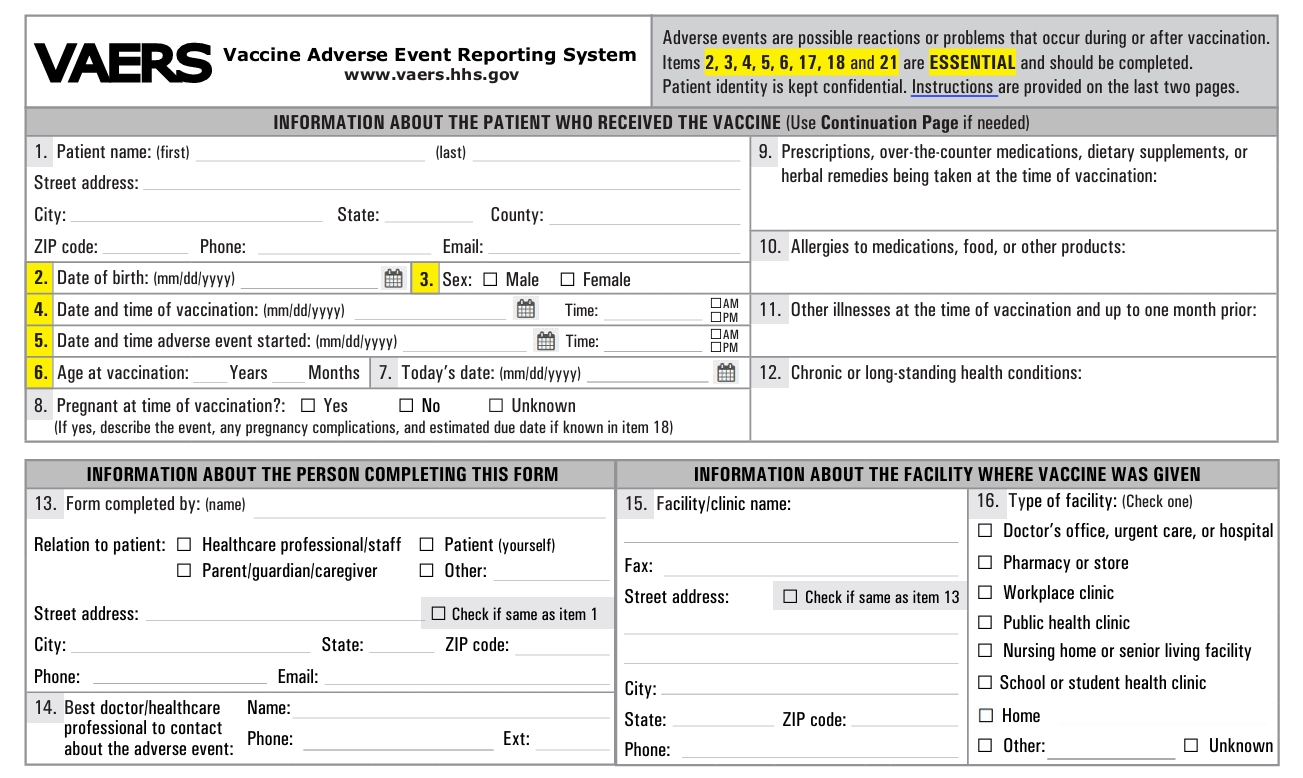
\includegraphics[scale=0.3]{Graphics/vaers_form.jpeg}
%     \caption{Ejemplo del formulario en formato PDF editable utilizado para el reporte de eventos adversos en el sistema VAERS}
%     \label{fig:figura2}
% \end{figure}

% \begin{figure}[htbp]
%     \centering
%     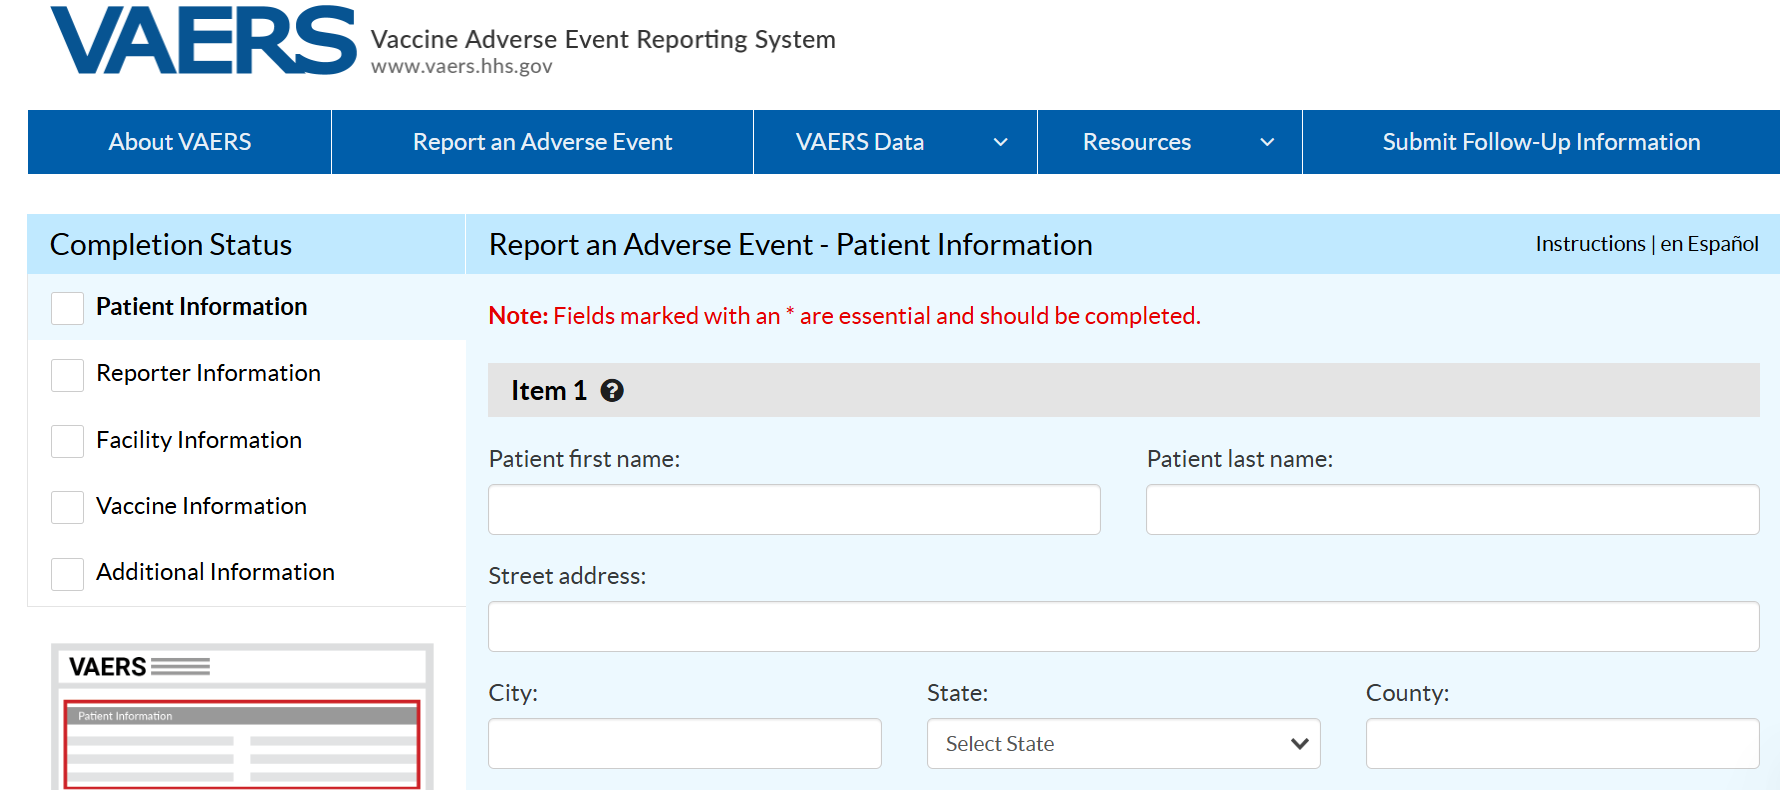
\includegraphics[scale=0.5]{Graphics/vaers_web_form.png}
%     \caption{Ejemplo del formulario web utilizado para el reporte de eventos adversos en el sistema VAERS}
%     \label{fig:figura3}
% \end{figure}

% % Fortalezas del sistema
% Entre las principales fortalezas de VAERS se encuentra su capacidad para actuar como un sistema de alerta temprana en la detección de eventos adversos poco frecuentes o inesperados. 
% Asimismo, su carácter abierto permite la participación de múltiples actores, incrementando la cantidad de información disponible para el análisis \cite{cdc_vaers}. 
% Adicionalmente, los datos recopilados son accesibles públicamente, lo que contribuye a la transparencia en la vigilancia de la seguridad vacunal.

% % Limitaciones del sistema
% No obstante, VAERS presenta limitaciones inherentes a los sistemas de vigilancia pasiva. 
% Entre ellas se encuentran el subregistro de eventos, la variabilidad en la calidad de los datos reportados y la posible existencia de sesgos de notificación \cite{cdc_vaers}. 
% Además, los reportes no permiten establecer relaciones causales directas entre la vacuna y el evento adverso, ya que muchos de estos pueden ocurrir de manera coincidente tras la inmunización \cite{fda_vaers}. 
% En este sentido \textquote{Tras realizar investigaciones, los científicos concluyen que la mayoría de los eventos notificados al VAERS no están asociados con la vacunación} (traducción propia) \cite{cdc_vaers}.
% Estas limitaciones requieren que los posibles riesgos identificados sean evaluados mediante sistemas complementarios y estudios más rigurosos, evidenciando la necesidad de enfoques más robustos en el diseño de sistemas de farmacovigilancia.

% \subsection{Sistema NotificaRAM de la Agencia Española de Medicamentos y Productos Sanitarios}

% \begin{figure}[htbp]
%     \centering
%     
\includegraphics[scale=0.3]{Graphics/Logo_notifica_ram.png}
%     \caption{Logotipo del sistema NotificaRAM (notificaram.es)}
%     \label{fig:figura4}
% \end{figure}

% % Descripción general
% El sistema \textbf{notificaRAM} constituye el formulario electrónico oficial de notificación de sospechas de reacciones adversas a medicamentos en España, permitiendo la comunicación de posibles efectos adversos por parte de ciudadanos y profesionales sanitarios \cite{aemps_manual_2025}. 
% Este formulario se integra en el Sistema Español de Farmacovigilancia de Medicamentos de Uso Humano (SEFV-H), una red nacional coordinada por la Agencia Española de Medicamentos y Productos Sanitarios (AEMPS) para la recogida, registro y evaluación de sospechas de reacciones adversas \cite{aemps_sefv_2025}.

% % Tipo de notificación
% El sistema se basa en un modelo de notificación espontánea, en el que las sospechas de reacciones adversas pueden ser comunicadas tanto por profesionales sanitarios como por la ciudadanía \cite{aemps_notificacion_2026}. 
% Los profesionales sanitarios deben notificar estas sospechas cuando las detectan, mientras que la ciudadanía puede hacerlo cuando sospecha una posible reacción adversa \cite{aemps_notificacion_2026}.

% % Actores que reportan
% Los actores implicados en la notificación incluyen profesionales sanitarios (como médicos, farmacéuticos y personal de enfermería) y ciudadanos o pacientes. 
% Ambos grupos pueden comunicar sospechas de reacciones adversas mediante los formularios disponibles en la plataforma \cite{aemps_manual_2025, aemps_notificacion_2026}.

% % Canal de notificación
% La notificación se realiza a través de formularios electrónicos disponibles en la plataforma oficial \url{https://www.notificaram.es}, donde el usuario selecciona el tipo de formulario según sea ciudadano o profesional sanitario. 
% Las notificaciones son remitidas a los centros autonómicos de farmacovigilancia para su evaluación e incorporación al sistema \cite{aemps_manual_2025, aemps_sefv_2025}.

% % Infraestructura del sistema
% El SEFV-H es una red descentralizada en la que los centros autonómicos de farmacovigilancia registran y evalúan las sospechas de reacciones adversas en una base de datos común denominada \textbf{FEDRA} (Farmacovigilancia Española, Datos de Reacciones Adversas) \cite{aemps_fedra_2026}. 
% Este sistema permite la recogida y análisis coordinado de las notificaciones dentro del sistema nacional de farmacovigilancia \cite{aemps_sefv_2025}.

% Asimismo, los casos registrados en FEDRA son transmitidos a la base de datos europea de sospechas de reacciones adversas \textbf{EudraVigilance}, utilizada por las agencias reguladoras de la Unión Europea para la detección de señales de seguridad \cite{aemps_notificacion_2026}.

% % Limitaciones
% El sistema presenta limitaciones propias del modelo de notificación espontánea, ya que la información depende de las sospechas comunicadas por los notificadores y de la calidad de los datos registrados \cite{aemps_notificacion_2026}. 
% En este sentido, pueden existir problemas de infranotificación, especialmente en casos leves o no reconocidos como reacciones adversas, así como variabilidad en la completitud y precisión de la información reportada. 
% Asimismo, la dependencia de la iniciativa del notificador introduce posibles sesgos, condicionados por factores como la experiencia clínica, el nivel de conocimiento del sistema o la percepción de gravedad del evento adverso.
% Adicionalmente, al no tratarse de un sistema de vigilancia activa, la capacidad para identificar de manera oportuna eventos poco frecuentes o establecer relaciones causales directas entre el medicamento y la reacción adversa puede verse limitada, requiriendo la realización de estudios complementarios más rigurosos.

% % \begin{figure}[htbp]
% %     \centering
% %     \includegraphics[scale=1.8]{Graphics/logo_aemps.jpg}
% %     \caption{Logotipo del sistema NotificaRAM (notificaram.es)}
% %     \label{fig:figura4}
% % \end{figure}

% \subsection{Sistema V-safe del Centers for Disease Control and Prevention}


% \begin{figure}[htbp]
%     \centering
%     
\includegraphics[scale=0.5]{Graphics/v-safe-logo.png}
%     \caption{Logotipo del sistema V-safe (vsafe.cdc.gov)}
%     \label{fig:figura5}
% \end{figure}


% El sistema \textbf{V-safe} es una herramienta digital de monitoreo de seguridad vacunal desarrollada por el \textit{Centers for Disease Control and Prevention} (CDC), orientada al seguimiento de personas vacunadas en los Estados Unidos.
% Se lanzó originalmente en diciembre de 2020 para monitorear la seguridad de las vacunas contra el \textbf{COVID-19}. 
% Ahora, V-safe permite rastrear a sujetos vacunados después de recibir una vacuna contra el COVID-19 o contra el \textbf{Virus Respiratorio Sincitial} (VRS)\cite{cdc_about_vsafe}. 

% A diferencia de los sistemas tradicionales de farmacovigilancia basados en notificación espontánea, V-safe implementa un enfoque de \textbf{vigilancia activa}, en el cual el sistema contacta de manera proactiva a los usuarios mediante encuestas periódicas enviadas tras la vacunación. 
% Después de inscribirse y seleccionar la vacuna que recibió, V-safe hace preguntas por mensajes de texto (SMS) o correo electrónico sobre cómo se siente el sujeto después de la vacunación, incluso si no presenta efectos secundarios. 
% De este modo, el sistema está dirigido principalmente a personas vacunadas que participan de forma voluntaria, permitiendo la recopilación sistemática de información directamente desde el usuario.
% Recibe un chequeo diario durante la primera semana, y luego un chequeo semanal durante seis semanas adicionales \cite{cdc_vsafe_portal}.

% La Figura \ref{fig:vsafe_flujo} muestra un ejemplo del flujo de interacción del sistema V-safe, donde se ilustra el proceso de envío de encuestas y la recolección de información por parte de los usuarios \cite{vsafe_monitoring_article}.

% \begin{figure}[htbp]
%     \centering
%     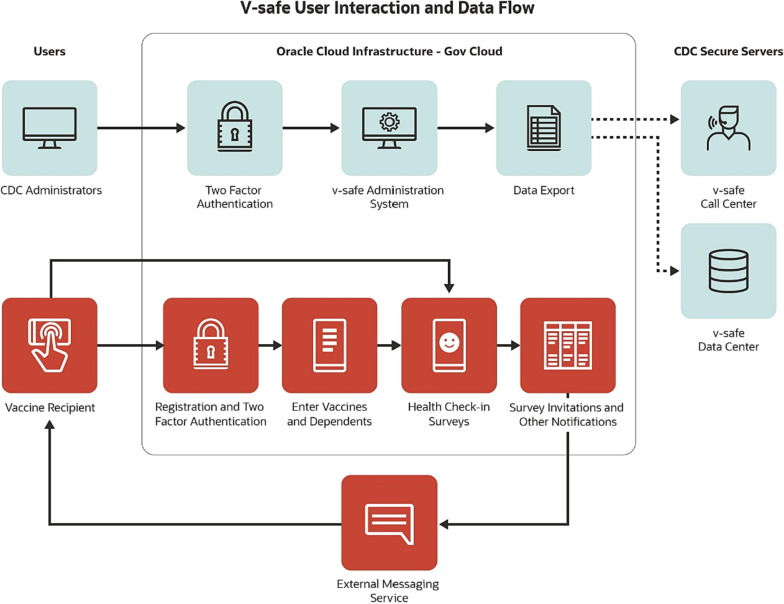
\includegraphics[scale=2.5]{Graphics/gr1_lrg.jpg}
%     \caption{Ejemplo del flujo de interacción del sistema V-safe mediante encuestas digitales}
%     \label{fig:vsafe_flujo}
% \end{figure}


% Desde una perspectiva funcional, una de las principales fortalezas de V-safe radica en su capacidad para implementar un modelo de vigilancia activa a gran escala, permitiendo la recopilación de datos en tiempo casi real sobre la seguridad de las vacunas. Durante su implementación inicial, el sistema demostró un alcance masivo: "más de 10 millones de personas se registraron y completaron más de 151 millones de encuestas" \cite{vsafe_monitoring_article}. Este enfoque permite al CDC comprender mejor los efectos secundarios experimentados poco después de la inmunización, aportando datos que a menudo superan los obtenidos en ensayos clínicos tradicionales.
% El diseño del sistema facilita un seguimiento longitudinal riguroso de los individuos vacunados. Esto se logra mediante un esquema de comunicación automatizado donde el usuario recibe un "chequeo de salud diario durante la primera semana después de la vacunación y luego un chequeo semanal por seis semanas adicionales". Esta periodicidad mejora la detección temprana de posibles eventos adversos y permite una observación continuada de la salud del paciente.
% Asimismo, la estandarización de las encuestas y el uso de tecnologías móviles (mensajes de texto y correos electrónicos) garantizan la obtención de datos estructurados y comparables. Al emplear herramientas digitales para realizar "chequeos que típicamente toman menos de dos minutos", el sistema optimiza la recolección de información técnica que ya ha sido utilizada en más de 25 publicaciones científicas para validar la seguridad de las vacunas \cite{vsafe_monitoring_article}

% No obstante, el sistema presenta limitaciones asociadas a su diseño y funcionamiento. 
% Entre ellas se encuentra la dependencia del acceso a dispositivos móviles y conectividad, lo cual puede generar sesgos en la población participante. 
% Asimismo, al tratarse de un sistema basado en autodeclaración, la información reportada puede carecer de validación clínica directa. 
% Adicionalmente, la participación voluntaria y longitudinal (que dura 6 semanas o más) fatiga al participante, un fenómeno documentado donde la respuesta suele decaer tras los primeros días. 
% Finalmente, aunque el sistema permite identificar patrones y señales de seguridad, no es suficiente por sí solo para establecer relaciones causales entre la vacunación y los eventos adversos reportados.


% \subsection{Análisis comparativo de los sistemas estudiados}

% El análisis de los sistemas VAERS, V-safe y NotificaRAM permite identificar diferencias significativas en cuanto a su enfoque metodológico, nivel de digitalización y mecanismos de captura de información.

% En primer lugar, se observa una distinción clara en el modelo de vigilancia implementado. VAERS y NotificaRAM se basan en esquemas de vigilancia pasiva, donde la calidad y cantidad de los datos dependen de la iniciativa de los notificadores. En contraste, V-safe adopta un enfoque de vigilancia activa, permitiendo la recolección sistemática y periódica de información directamente desde los usuarios vacunados.

% Desde la perspectiva tecnológica, V-safe presenta un mayor grado de digitalización al integrar mecanismos automatizados de seguimiento mediante dispositivos móviles, lo que facilita la interacción continua con el usuario. Por su parte, VAERS y NotificaRAM, aunque disponen de plataformas web, dependen en mayor medida de la acción voluntaria del usuario para el envío de reportes.

% En cuanto a los actores involucrados, los sistemas pasivos permiten una mayor diversidad de notificadores, incluyendo profesionales de la salud, fabricantes y ciudadanos. Sin embargo, esta apertura introduce variabilidad en la calidad de los datos. En contraste, V-safe se centra en usuarios previamente registrados, lo que permite una mayor consistencia en la información recolectada.

% Finalmente, en términos de limitaciones, los sistemas de vigilancia pasiva presentan problemas de subregistro, sesgos de notificación y dificultades para establecer relaciones causales. Por otro lado, aunque V-safe mejora la calidad y frecuencia de los datos, su alcance se limita a los usuarios que participan voluntariamente en el sistema.

% En conjunto, estos sistemas reflejan diferentes enfoques dentro de la farmacovigilancia moderna, evidenciando un tránsito desde modelos reactivos hacia estrategias más proactivas y centradas en el usuario.

% \subsection{Conclusiones sobre las soluciones actuales}

% El estudio de los sistemas analizados evidencia que, si bien existen soluciones consolidadas para la notificación de eventos adversos, estas presentan limitaciones significativas desde el punto de vista funcional y tecnológico.

% Los sistemas basados en vigilancia pasiva, como VAERS y NotificaRAM, continúan siendo fundamentales debido a su amplia cobertura y apertura a múltiples actores. No obstante, su dependencia de la notificación voluntaria limita la completitud, oportunidad y calidad de los datos recolectados.

% Por otro lado, soluciones más recientes como V-safe introducen enfoques innovadores basados en vigilancia activa y tecnologías móviles, mejorando la frecuencia y consistencia de la información. Sin embargo, estos sistemas presentan restricciones en términos de alcance poblacional y dependencia de la participación voluntaria de los usuarios.

% De manera general, se identifica la necesidad de sistemas que integren las ventajas de ambos enfoques, combinando la accesibilidad y cobertura de la vigilancia pasiva con mecanismos automatizados que permitan una recolección más sistemática, oportuna y estructurada de los datos.

% Estas limitaciones evidencian oportunidades para el diseño de nuevas soluciones tecnológicas orientadas a mejorar la eficiencia, calidad e interoperabilidad en la notificación de eventos adversos, lo cual constituye la base para el desarrollo del sistema propuesto en la presente investigación.


% \section{Análisis de tecnologías para la implementación del sistema propuesto}
% \label{section:analisis_tecnologias}

% El desarrollo de sistemas informáticos modernos orientados al dominio clínico requiere la selección de un conjunto de tecnologías que garanticen propiedades fundamentales como la confiabilidad, la integridad de los datos, la escalabilidad y la mantenibilidad del software. A diferencia de aplicaciones convencionales, en este tipo de sistemas resulta especialmente relevante la correcta gestión de la información, así como la capacidad de respuesta ante un crecimiento progresivo de usuarios y volumen de datos.

% En este sentido, el presente análisis se basa en el estudio de diferentes alternativas tecnológicas utilizadas en la construcción de sistemas modernos, abarcando tanto el desarrollo del backend como de las interfaces de usuario y los sistemas de gestión de bases de datos. La selección de estas tecnologías no se realiza de manera arbitraria, sino a partir de criterios técnicos previamente definidos que permiten evaluar de forma objetiva las distintas opciones disponibles.

% \subsection{Criterios técnicos para la selección de tecnologías}
% \label{subsection:criterios}

% Con el objetivo de realizar una selección fundamentada de las tecnologías que conformarán la solución propuesta, se definen criterios de evaluación orientados a las necesidades de sistemas clínicos.

% En primer lugar, se considera la \textbf{eficiencia y el rendimiento}, entendidos como la capacidad de la tecnología para responder adecuadamente bajo cargas de trabajo variables, garantizando tiempos de respuesta adecuados en escenarios de uso intensivo.

% En segundo lugar, se evalúa la \textbf{escalabilidad}, referida a la capacidad del sistema para adaptarse al crecimiento en el número de usuarios y volumen de datos, tanto a nivel vertical como horizontal.

% Asimismo, se analiza la \textbf{mantenibilidad},  entendida como la facilidad para realizar modificaciones, extensiones o correcciones en el software sin afectar negativamente su funcionamiento global, en función del nivel de acoplamiento y la estructura arquitectónica.

% Otro criterio considerado es la \textbf{madurez tecnológica}, entendida como el nivel de estabilidad y uso comprobado de una tecnología, reflejado en su adopción en entornos reales, la calidad de su documentación y el soporte de su comunidad.

% Finalmente, se introduce el criterio de \textbf{adecuación al dominio clínico}, el cual evalúa la capacidad de la tecnología para garantizar propiedades críticas como la consistencia de los datos, la trazabilidad de la información y el soporte de operaciones transaccionales seguras.

% Estos criterios constituyen la base para el análisis comparativo presentado en las secciones siguientes.


% \subsection{Tecnologías para el desarrollo del backend}
% \label{subsection:backend}

% \subsubsection{.NET Core}

% \begin{figure}[htbp]
%     \centering
%     
\includegraphics[scale=0.8]{Graphics/dotnetcore-original.png}
%     \caption{Logo de .NET.}
%     \label{fig:dotnet_core}
% \end{figure}

% .NET Core (actualmente integrado dentro de la plataforma unificada .NET 6+) es un framework de desarrollo multiplataforma, de código abierto, mantenido por Microsoft \cite{dotnet_official}, orientado a la construcción de aplicaciones modernas, incluyendo servicios web, APIs REST y aplicaciones de alto rendimiento. 
% Su diseño modular y su enfoque en la eficiencia lo convierten en una alternativa adecuada para el desarrollo de sistemas backend que requieren confiabilidad y escalabilidad.

% Una de las principales características de la plataforma .NET es su modelo de ejecución basado en el Common Language Runtime (CLR), el cual proporciona un entorno gestionado para la ejecución del código, permitiendo un manejo eficiente de la memoria, control de excepciones y seguridad en tiempo de ejecución \cite{dotnet_official}.

% El framework proporciona soporte nativo para la construcción de servicios web mediante ASP.NET Core, facilitando el desarrollo de APIs REST con una arquitectura desacoplada y orientada a servicios \cite{ms_aspnet_architecture}. 
% Este enfoque contribuye a la separación de responsabilidades dentro del sistema, favoreciendo la mantenibilidad y la evolución del software.

% Asimismo, .NET integra herramientas como Entity Framework Core, que permiten interactuar con bases de datos relacionales mediante un enfoque orientado a objetos \cite{dotnet_official}. 
% Este mecanismo simplifica el acceso a datos y facilita la implementación de operaciones transaccionales, contribuyendo a la consistencia de la información en sistemas que gestionan datos críticos.

% Adicionalmente, la plataforma se integra con patrones de diseño ampliamente utilizados en el desarrollo de software moderno, tales como la arquitectura en capas, el patrón MVC y la inyección de dependencias, lo cual favorece la construcción de sistemas escalables y mantenibles \cite{ms_aspnet_architecture}.

% Desventajas:
% \begin{itemize}
%     \item Dependencia del ecosistema Microsoft, lo cual puede limitar la portabilidad en ciertos contextos tecnológicos.
%     \item Menor flexibilidad en la integración con herramientas fuera del entorno .NET en comparación con otras alternativas.
%     \item Curva de aprendizaje asociada a la comprensión del ecosistema completo (.NET, ASP.NET, Entity Framework).
%     \item Requiere una correcta estructuración inicial para aprovechar adecuadamente sus capacidades arquitectónicas.
% \end{itemize}


% \subsubsection{Spring Boot}

% \begin{figure}[htbp]
%     \centering
%     
\includegraphics[scale=0.8]{Graphics/spring-original.png}
%     \caption{Logo de Spring Boot}
%     \label{fig:spring_boot}
% \end{figure}

% Spring Boot es un framework de desarrollo basado en Java, de código abierto, mantenido por VMware, orientado a la construcción de aplicaciones backend modernas, incluyendo servicios web, APIs REST y aplicaciones empresariales escalables \cite{spring_official}. 
% Su enfoque en la configuración automática y la reducción de complejidad en la inicialización de proyectos lo convierten en una alternativa ampliamente utilizada en el desarrollo de sistemas robustos.

% Una de las principales características del ecosistema Spring es su modelo basado en la Inversión de Control (IoC), implementado a través de un contenedor que gestiona el ciclo de vida de los componentes y sus dependencias \cite{spring_official}. 
% Este mecanismo permite desacoplar las distintas partes del sistema, facilitando la mantenibilidad y promoviendo buenas prácticas de diseño.

% El framework proporciona soporte para la construcción de servicios web mediante Spring MVC, lo cual permite el desarrollo de APIs REST siguiendo un enfoque basado en controladores y patrones bien definidos \cite{spring_in_action}.
% Este modelo favorece la separación de responsabilidades dentro del sistema y contribuye a una organización estructurada del código.

% Asimismo, Spring Boot integra herramientas como Spring Data, que permiten la interacción con bases de datos relacionales mediante abstracciones de alto nivel \cite{spring_official}.
% Este enfoque simplifica el acceso a datos y facilita la implementación de operaciones transaccionales, contribuyendo a la consistencia de la información en sistemas que manejan datos críticos.

% Adicionalmente, el modelo basado en inversión de control permite una gestión flexible de las dependencias entre componentes, facilitando la extensibilidad del sistema y su adaptación a cambios en los requisitos \cite{spring_in_action}.

% Desventajas:
% \begin{itemize}
%     \item Complejidad conceptual asociada al modelo de inversión de control y al uso extensivo de anotaciones, lo cual puede dificultar la comprensión del flujo de ejecución del sistema.
%     \item Mayor esfuerzo inicial requerido para estructurar correctamente la aplicación, especialmente en sistemas con múltiples módulos.
%     \item Posibilidad de introducir errores de configuración si no se gestiona adecuadamente el ciclo de vida de los componentes.
%     \item Verbosidad inherente al lenguaje Java, lo cual puede afectar la productividad en comparación con alternativas más concisas.
% \end{itemize}


% \subsubsection{NestJS}

% \begin{figure}[htbp]
%     \centering
%     
\includegraphics[scale=0.8]{Graphics/nestjs-original.png}
%     \caption{Logo de NestJS}
%     \label{fig:nest_js}
% \end{figure}

% NestJS es un framework de desarrollo backend basado en Node.js y TypeScript, de código abierto, diseñado para la construcción de aplicaciones escalables y mantenibles \cite{nestjs_official}. 
% Su arquitectura está fuertemente inspirada en patrones como la inversión de control y la programación modular, lo cual permite estructurar aplicaciones de manera organizada y predecible.

% Una de sus principales características es el uso intensivo de TypeScript, lo cual introduce tipado estático en el desarrollo sobre Node.js, favoreciendo la detección temprana de errores y mejorando la mantenibilidad del código.

% El framework implementa un sistema de inyección de dependencias similar al de otros frameworks modernos, permitiendo desacoplar componentes y facilitar la prueba y reutilización del código \cite{nestjs_official}.

% Asimismo, NestJS utiliza una arquitectura basada en módulos, controladores y servicios, lo cual permite organizar la lógica de negocio de manera estructurada, similar a patrones utilizados en frameworks como Spring Boot o ASP.NET Core.
% Adicionalmente, NestJS puede integrarse con bibliotecas de persistencia de datos como TypeORM o Prisma, lo cual permite la interacción con bases de datos relacionales mediante un enfoque basado en entidades o esquemas tipados, dependiendo de la implementación seleccionada.

% Desventajas:
% \begin{itemize}
%     \item Menor madurez en entornos empresariales críticos en comparación con frameworks como Spring Boot o .NET.
%     \item Dependencia del ecosistema Node.js, lo cual puede introducir variabilidad en la gestión de dependencias.
%     \item Rendimiento dependiente del runtime de JavaScript/Node en comparación con soluciones compiladas.
%     \item Comunidad y ecosistema aún en crecimiento en comparación con alternativas más consolidadas.
% \end{itemize}

% \subsection{Conclusiones sobre las plataformas de desarrollo expuestas}

% A partir del análisis realizado, se evidencia que las tres tecnologías estudiadas presentan enfoques válidos para el desarrollo de aplicaciones backend modernas, con características que responden a distintos paradigmas de diseño y necesidades de implementación.

% .NET Core destaca por su integración con el ecosistema Microsoft y su fuerte soporte para aplicaciones empresariales con altos requerimientos de confiabilidad y consistencia de datos. 
% Por su parte, Spring Boot ofrece un modelo de desarrollo basado en la inversión de control que favorece la flexibilidad y la organización modular del sistema. 
% En contraste, NestJS representa una alternativa moderna dentro del ecosistema Node.js, caracterizada por el uso de TypeScript y una arquitectura inspirada en patrones ampliamente utilizados en frameworks empresariales.

% En función del contexto del sistema propuesto, orientado a la gestión de información sensible en el ámbito de la salud, se identifican como aspectos relevantes la robustez del modelo de persistencia de datos, el soporte para arquitecturas estructuradas y la madurez del ecosistema tecnológico. 
% Estos elementos serán tomados como base para la selección de las tecnologías que conformarán la solución final del sistema.


% %-------------------------------------------------

% \subsection{Tecnologías para el desarrollo del frontend}
% \label{subsection:frontend}

% \subsubsection{React}

% \begin{figure}[htbp]
%     \centering
%     
\includegraphics[scale=0.8]{Graphics/react-original-wordmark.png}
%     \caption{Logo de React}
%     \label{fig:react}
% \end{figure}

% React es una biblioteca de JavaScript de código abierto desarrollada por Meta, orientada a la construcción de interfaces de usuario basadas en componentes reutilizables. Su paradigma declarativo permite describir el estado de la interfaz y delegar la actualización del DOM a un mecanismo eficiente de reconciliación \cite{react_official}.

% Una de sus principales características es el uso de un Virtual DOM, lo cual optimiza las actualizaciones de la interfaz al minimizar operaciones directas sobre el DOM real. Este enfoque resulta especialmente útil en aplicaciones con alta interacción del usuario y cambios frecuentes en la interfaz.

% Adicionalmente, React puede ser complementado con TypeScript, lo cual introduce tipado estático y mejora la mantenibilidad del código en sistemas de mediana y gran escala.

% Sin embargo, React no constituye una solución completa por sí misma, ya que requiere la integración de librerías externas para aspectos como enrutamiento, gestión de estado y arquitectura de la aplicación, lo cual puede incrementar la complejidad del ecosistema.

% \subsubsection{Angular}

% \begin{figure}[htbp]
%     \centering
%     
\includegraphics[scale=0.8]{Graphics/angularjs-original.png}
%     \caption{Logo de Angular}
%     \label{fig:angular}
% \end{figure}

% Angular es un framework de desarrollo frontend basado en TypeScript, mantenido por Google, orientado a la construcción de aplicaciones web de gran escala. A diferencia de bibliotecas como React, Angular proporciona una solución integral que incluye enrutamiento, inyección de dependencias, manejo de formularios y herramientas de estructuración de aplicaciones \cite{angular_official}.

% Su arquitectura basada en componentes y módulos permite organizar el código de manera estructurada, favoreciendo la escalabilidad en proyectos complejos. Además, su sistema de inyección de dependencias facilita la modularidad y la reutilización de componentes.

% No obstante, Angular introduce una curva de aprendizaje más pronunciada debido a la cantidad de conceptos integrados en el framework, así como una mayor complejidad inicial en comparación con alternativas más ligeras.

% \subsubsection{Vue}

% \begin{figure}[htbp]
%     \centering
%     
\includegraphics[scale=0.8]{Graphics/vuejs-original-wordmark.png}
%     \caption{Logo de Vue.js}
%     \label{fig:vue}
% \end{figure}

% Vue.js es un framework progresivo de JavaScript diseñado para la construcción de interfaces de usuario interactivas. Su diseño incremental permite su adopción gradual, integrándose fácilmente en proyectos existentes o utilizándose como framework completo en aplicaciones modernas \cite{vue_official}.

% Vue combina características de frameworks como Angular y React, ofreciendo un sistema de reactividad eficiente y una sintaxis accesible para el desarrollo de interfaces declarativas.

% Sin embargo, aunque su ecosistema ha crecido considerablemente, en entornos empresariales de gran escala su adopción es menor en comparación con Angular o React, lo cual puede influir en la disponibilidad de recursos y soporte a largo plazo.


% \subsection{Conclusiones sobre los frameworks de frontend expuestos}

% A partir del análisis realizado, se observa que React, Angular y Vue representan enfoques distintos para la construcción de interfaces de usuario modernas.

% React destaca por su flexibilidad y su amplio ecosistema, permitiendo la construcción de interfaces altamente dinámicas mediante un enfoque basado en componentes. 
% Angular, por su parte, proporciona una solución más estructurada e integral, adecuada para aplicaciones de gran escala que requieren una arquitectura estricta desde el inicio. 
% Vue se posiciona como una alternativa intermedia, con una curva de aprendizaje más suave y un enfoque progresivo.

% En el contexto del sistema propuesto, caracterizado por interfaces altamente interactivas basadas en formularios dinámicos, se considera adecuado el uso de un enfoque basado en componentes con alta reactividad, lo cual favorece la elección de React como tecnología base para el desarrollo del frontend.



% %-------------------------------------------------

% \subsection{Sistemas de gestión de bases de datos}
% \label{subsection:bases_datos}

% \subsubsection{Bases de datos relacionales}

% \begin{figure}[htbp]
%     \centering
%     
\includegraphics[scale=0.8]{Graphics/mysql-original-wordmark.png}
%     \caption{Sistema de gestión de bases de datos relacionales : MySQL}
%     \label{fig:mysql}
% \end{figure}

% Las bases de datos relacionales constituyen un modelo de almacenamiento de información basado en estructuras tabulares compuestas por filas y columnas, donde las relaciones entre entidades se establecen mediante claves primarias y foráneas. 
% Este enfoque permite garantizar propiedades fundamentales como la integridad referencial, la consistencia de los datos y el cumplimiento de transacciones ACID, aspectos críticos en sistemas que gestionan información sensible o estructurada \cite{elmasri2016fundamentals}.

% MySQL es uno de los sistemas de gestión de bases de datos relacionales más ampliamente utilizados en el desarrollo de aplicaciones web y empresariales, caracterizado por su madurez, rendimiento y amplio soporte comunitario \cite{mysql_official}. 
% Su modelo relacional facilita la implementación de esquemas bien definidos, lo cual resulta adecuado en escenarios donde la coherencia de los datos es un requisito prioritario, como es el caso de sistemas clínicos o de registro estructurado de eventos.

% Sin embargo, este tipo de sistemas puede presentar limitaciones en contextos donde se requiere una alta flexibilidad en la estructura de los datos o una escalabilidad horizontal intensiva, debido a la rigidez inherente del modelo relacional y a la necesidad de mantener esquemas previamente definidos.

% \subsubsection{Bases de datos NoSQL}


% \begin{figure}[htbp]
%     \centering
%     
\includegraphics[scale=0.8]{Graphics/mongodb-original-wordmark.png}
%     \caption{Sistema de gestión de bases de datos no relacionales : MongoDB}
%     \label{fig:mongodb}
% \end{figure}


% Las bases de datos NoSQL surgen como alternativa a los modelos relacionales tradicionales, con el objetivo de ofrecer mayor flexibilidad en la estructura de los datos y una mejor adaptación a entornos distribuidos y de gran escala. 
% A diferencia del modelo relacional, estas bases de datos no requieren un esquema rígido, lo que permite la gestión de datos semi-estructurados o no estructurados \cite{moniruzzaman2013nosql}.

% MongoDB es uno de los sistemas NoSQL más representativos, basado en un modelo de documentos que almacena la información en formato BSON. 
% Este enfoque permite una evolución más dinámica del esquema de datos y facilita la escalabilidad horizontal en sistemas con grandes volúmenes de información \cite{mongodb_official}.

% No obstante, la flexibilidad del modelo NoSQL puede implicar desafíos en la consistencia de los datos y en la gestión de relaciones complejas entre entidades, lo cual puede resultar una limitación en sistemas donde la integridad de la información es un requisito crítico, como en aplicaciones de dominio clínico o regulado.

% \subsection{Conclusiones sobre los sistemas de gestión de bases de datos expuestos}

% A partir del análisis realizado, se evidencia que los sistemas de gestión de bases de datos relacionales y NoSQL responden a paradigmas distintos de modelado y almacenamiento de la información, los cuales se adaptan a necesidades específicas de cada tipo de sistema.

% Las bases de datos relacionales, representadas en este análisis por sistemas como MySQL, se caracterizan por un modelo estructurado basado en tablas y relaciones explícitas, lo cual permite garantizar propiedades como la integridad referencial, la consistencia de los datos y el soporte de transacciones ACID. 
% Estas características resultan especialmente relevantes en sistemas que requieren alta confiabilidad en la gestión de información estructurada, como es el caso de aplicaciones en el dominio clínico.

% Por otra parte, las bases de datos NoSQL, representadas por sistemas como MongoDB, ofrecen un modelo de almacenamiento más flexible, orientado a documentos, lo cual facilita la evolución dinámica del esquema de datos y la escalabilidad horizontal en entornos distribuidos. 
% Sin embargo, esta flexibilidad puede implicar compromisos en términos de consistencia fuerte y en la gestión de relaciones complejas entre entidades.

% En función del contexto del sistema propuesto, donde la integridad de los datos, la trazabilidad de eventos y la consistencia de la información constituyen requisitos fundamentales, se considera que los sistemas relacionales presentan ventajas significativas para la implementación de la solución.

% %-------------------------------------------------

% \subsection{Síntesis comparativa de las tecnologías analizadas}
% \label{subsection:sintesis}

% A partir del análisis realizado en las secciones anteriores, se evidencia que las tecnologías evaluadas presentan características diferenciadas en función del componente del sistema al que están orientadas, así como de los paradigmas de diseño que promueven.

% En el ámbito del backend, se identifican soluciones orientadas a la construcción de sistemas robustos y mantenibles, destacándose plataformas consolidadas como .NET y Spring Boot por su madurez, soporte arquitectónico y enfoque en aplicaciones empresariales, así como alternativas más recientes como NestJS, que introducen modelos modulares y flexibles dentro del ecosistema JavaScript.

% En cuanto al desarrollo de interfaces de usuario, se observa una tendencia hacia arquitecturas basadas en componentes y modelos declarativos, donde tecnologías como React, Angular y Vue ofrecen distintos niveles de estructuración, flexibilidad y control sobre la complejidad de la aplicación, en función de los requerimientos de interacción y dinamismo de la interfaz.

% Por otra parte, en el contexto de la persistencia de datos, las tecnologías analizadas reflejan enfoques diferenciados en cuanto al modelado y gestión de la información, lo cual influye directamente en aspectos como la consistencia, la integridad y la adaptabilidad del sistema ante cambios en los datos.

% De manera integral, se evidencia que la selección tecnológica no debe realizarse de forma aislada por componente, sino considerando la coherencia entre las distintas capas del sistema. En particular, la combinación de tecnologías backend, frontend y de persistencia debe garantizar un equilibrio entre rendimiento, mantenibilidad y confiabilidad, aspectos especialmente críticos en sistemas orientados a la gestión de información clínica.

% Estos elementos constituyen la base para la selección de las tecnologías que serán empleadas en la implementación del sistema, la cual se aborda en el capítulo siguiente.


% \section{Tecnologías y enfoques para la gestión de datos clínicos}
% \label{section:tecnologias_datos_clinicos}

% La gestión de datos clínicos en sistemas de farmacovigilancia constituye un problema de naturaleza compleja, en el cual convergen requisitos de interoperabilidad semántica, consistencia estructural, trazabilidad de la información y calidad en la captura de los datos. 
% A diferencia de los sistemas de información convencionales, los entornos clínicos demandan un tratamiento riguroso de la información debido a su impacto directo en procesos de análisis sanitario, toma de decisiones en salud pública y evaluación de la seguridad de las vacunas.

% En este contexto, los enfoques tecnológicos asociados a la gestión de datos clínicos no se limitan únicamente a herramientas de almacenamiento o procesamiento, sino que abarcan también estándares de representación de la información, modelos de captura de datos y mecanismos de validación que permiten garantizar la integridad de los registros desde su origen hasta su utilización en procesos analíticos.

% Asimismo, la heterogeneidad de las fuentes de datos y la variabilidad en la forma en que los usuarios reportan eventos adversos introduce el denominado problema de “ruido informativo”, el cual dificulta la integración y el análisis automatizado de la información clínica. 
% Por esta razón, resulta necesario el uso de estándares y enfoques que permitan normalizar la representación de los datos, así como establecer reglas de validación que aseguren su coherencia y fiabilidad.

% De igual forma, los sistemas de farmacovigilancia modernos han evolucionado hacia modelos que combinan distintos paradigmas de captura de información, incluyendo mecanismos de reporte en línea y modelos de captura diferida mediante formularios estructurados, con el objetivo de garantizar la disponibilidad del sistema en escenarios con conectividad limitada sin comprometer la calidad de los datos recolectados.

% En las subsecciones siguientes se analizan los principales estándares internacionales utilizados en la representación de información clínica, los modelos de captura de datos empleados en sistemas de autorreporte de eventos adversos, así como los enfoques de validación de datos clínicos, con el objetivo de fundamentar las decisiones de diseño adoptadas en la presente investigación.




% \subsection{Estándares de interoperabilidad clínica}
% \label{subsection:interoperabilidad_clinica}

% La interoperabilidad en sistemas de información en salud constituye un requisito esencial para garantizar que los datos clínicos puedan ser compartidos, interpretados y reutilizados de manera consistente entre diferentes sistemas y actores del ecosistema sanitario. En el contexto de la farmacovigilancia de vacunas, esta capacidad resulta fundamental para asegurar que la información reportada mantenga su significado original y pueda ser utilizada de forma fiable en procesos de análisis y toma de decisiones.

% Uno de los estándares más relevantes en este ámbito es HL7 FHIR (Fast Healthcare Interoperability Resources), desarrollado por la organización HL7 \cite{hl7_fhir_official}, el cual define un modelo basado en recursos que permite estructurar la información clínica de manera modular e interoperable. 
% Este estándar facilita la representación de entidades como pacientes, vacunas administradas y eventos clínicos asociados, permitiendo la integración entre sistemas heterogéneos.

% El modelo basado en FHIR introduce una estructura flexible donde cada recurso representa una unidad de información clínica que puede ser combinada con otras para describir eventos complejos. En el caso de los eventos adversos asociados a vacunas, esta estructura permite relacionar el paciente, la inmunización recibida y las observaciones clínicas derivadas.

% Por otra parte, la estandarización terminológica constituye un elemento clave para evitar ambigüedades en la interpretación de los datos. En este sentido, el diccionario MedDRA (Medical Dictionary for Regulatory Activities) proporciona una terminología controlada para la codificación de eventos adversos \cite{meddra_official}, permitiendo la representación uniforme de síntomas y reacciones asociadas a vacunas.

% Como se observa en la Figura \ref{fig:meddra_hierarchy}, MedDRA organiza los términos clínicos en una estructura jerárquica de cinco niveles, que permite representar un mismo concepto clínico con distintos grados de especificidad. Esta jerarquía va desde categorías generales (System Organ Class) hasta términos altamente específicos (Lowest Level Term), lo cual facilita la normalización semántica de los eventos reportados y reduce la ambigüedad en la interpretación de los datos clínicos.

% \begin{figure}[htbp]
%     \centering
%     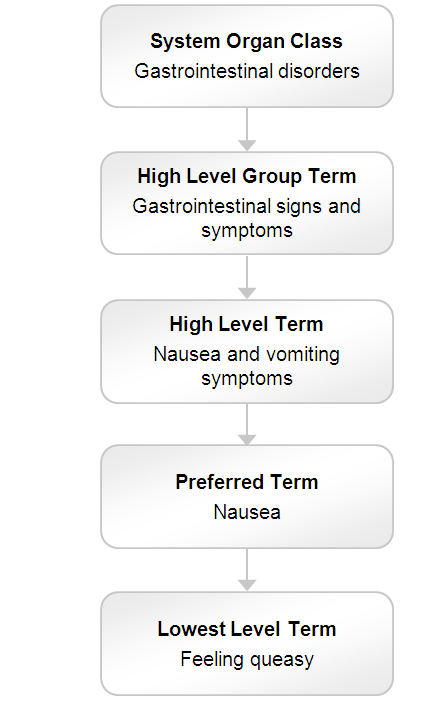
\includegraphics[scale=0.3]{Graphics/meddra_graph.png}
%     \caption{Estructura jerárquica del sistema de codificación MedDRA.}
%     \label{fig:meddra_hierarchy}
% \end{figure}

% De manera complementaria, la Clasificación Internacional de Enfermedades (CIE), desarrollada por la Organización Mundial de la Salud \cite{who_icd}, proporciona un marco estandarizado para la codificación de condiciones de salud, lo cual permite enriquecer el contexto clínico de los reportes cuando es necesario.

% En conjunto, la adopción de estándares de interoperabilidad y terminologías controladas como FHIR, MedDRA y CIE permite mejorar la calidad, consistencia y utilidad de los datos clínicos, constituyendo un elemento fundamental en el diseño de sistemas orientados al reporte estructurado de eventos adversos asociados a vacunas.


% \subsection{Modelos de captura de datos clínicos}

% La captura de datos clínicos constituye una etapa crítica en el diseño de sistemas de información en salud, ya que determina en gran medida la calidad, consistencia y utilidad de la información registrada. En el contexto de los sistemas de reporte de eventos adversos asociados a vacunas, una captura inadecuada puede derivar en pérdidas de información relevante, ambigüedades en los datos o dificultades en su posterior procesamiento.

% En la práctica, pueden identificarse diferentes modelos de captura de datos clínicos en función del nivel de estructuración de la información desde su origen.

% El modelo de captura estructurada se basa en la utilización de formularios con campos previamente definidos, lo cual permite restringir los valores de entrada y facilitar la validación automática de los datos. Este enfoque es ampliamente utilizado en sistemas de información en salud modernos, debido a su capacidad para mejorar la calidad del dato desde su origen y facilitar su procesamiento posterior.

% El modelo semi-estructurado constituye un enfoque intermedio, donde la información se organiza bajo una plantilla definida pero permite cierto grado de flexibilidad en su completitud. Un ejemplo representativo de este enfoque es el formulario en formato PDF utilizado en sistemas de farmacovigilancia como el Vaccine Adverse Event Reporting System (VAERS), el cual permite la recolección de información incluso en escenarios donde no existe conectividad continua o acceso a plataformas en línea \cite{vaers_official}.

% Finalmente, el modelo no estructurado se basa en la captura de información en forma de texto libre o descripciones narrativas. Aunque este enfoque puede aportar mayor riqueza descriptiva, presenta limitaciones significativas en términos de procesamiento automático, normalización de datos e integración con sistemas de análisis clínico.

% Desde la perspectiva del diseño de sistemas de información, los modelos estructurados y semi-estructurados resultan más adecuados para escenarios de farmacovigilancia, ya que permiten garantizar un mayor control sobre la calidad de los datos desde su origen, facilitando su integración con procesos posteriores de validación, normalización y análisis.

% En consecuencia, la selección del modelo de captura debe equilibrar la precisión de la información, la facilidad de uso para el usuario final y la capacidad de integración con los procesos de análisis del sistema.

% \subsection{Herramientas para la validación reactiva de formularios}

% La validación de datos en tiempo de captura constituye un mecanismo esencial para garantizar la calidad y consistencia de la información en sistemas de autorreporte clínico. En este contexto, la validación reactiva se refiere al proceso de verificación de los datos introducidos por el usuario de manera inmediata, es decir, antes de su envío al servidor, permitiendo detectar y corregir errores en etapas tempranas del flujo de interacción.

% Este tipo de validación resulta especialmente relevante en sistemas de reporte de eventos adversos asociados a vacunas, donde la precisión de los datos ingresados impacta directamente en la confiabilidad del análisis posterior.

% Las técnicas de validación pueden clasificarse en validaciones sintácticas, orientadas a verificar el formato de los datos (como fechas, números o identificadores), y validaciones semánticas básicas, enfocadas en garantizar coherencia lógica entre los campos del formulario. Ejemplos de estas incluyen la verificación de campos obligatorios, rangos válidos de valores o consistencia entre fechas relacionadas.

% En el desarrollo de aplicaciones modernas, existen múltiples herramientas que facilitan la implementación de validación reactiva. En el ecosistema frontend basado en React, bibliotecas como React Hook Form y Formik permiten gestionar formularios complejos con validación en tiempo real \cite{react_hook_form} \cite{formik_docs}. De manera similar, en Angular se emplean formularios reactivos que integran validación mediante el módulo Reactive Forms \cite{angular_forms}.

% En el ámbito del backend, frameworks como .NET incorporan bibliotecas como FluentValidation, que permiten definir reglas de validación de forma declarativa y reutilizable \cite{fluentvalidation_docs}. En ecosistemas basados en Node.js, bibliotecas como Joi o Zod proporcionan mecanismos de validación estructurada de datos antes de su persistencia.

% La utilización de estas herramientas permite reducir significativamente la probabilidad de inserción de datos inconsistentes, mejorando la calidad de la información desde su punto de origen y complementando los procesos posteriores de normalización e integración en el sistema.

% \subsection{Calidad e integración de datos clínicos}

% La calidad de los datos clínicos constituye un factor determinante en la utilidad de los sistemas de información en salud, especialmente en contextos donde la información es utilizada para el análisis de eventos adversos asociados a vacunas. En este tipo de sistemas, la presencia de datos incompletos, inconsistentes o ambiguos puede comprometer significativamente la fiabilidad de los resultados obtenidos.

% Desde una perspectiva de ingeniería de software, la calidad de los datos puede evaluarse a partir de múltiples dimensiones, entre las que se incluyen la integridad, la consistencia, la exactitud, la completitud y la trazabilidad. Estas propiedades garantizan que la información almacenada represente de manera fiel los eventos del mundo real y pueda ser utilizada de forma confiable en procesos posteriores de análisis.

% La integración de datos clínicos se refiere al proceso mediante el cual la información capturada y validada en el sistema es unificada bajo un modelo común, permitiendo su interoperabilidad y su posterior procesamiento. En este sentido, la utilización de un modelo de datos estructurado resulta esencial para evitar la fragmentación de la información y facilitar su análisis global.

% En el contexto de los sistemas de autorreporte de eventos adversos, la integración de datos se apoya en el uso de estándares de interoperabilidad como HL7 FHIR \cite{hl7_fhir_official}, que permite la representación estructurada de entidades clínicas, y en terminologías controladas como MedDRA \cite{meddra_official} y la Clasificación Internacional de Enfermedades (CIE) de la Organización Mundial de la Salud \cite{who_icd}, que aseguran la normalización semántica de los conceptos médicos.

% Estos estándares permiten establecer un lenguaje común entre sistemas heterogéneos, facilitando la interoperabilidad, la coherencia semántica de los datos y su reutilización en diferentes contextos clínicos.

% Asimismo, la integración adecuada de los datos clínicos permite establecer relaciones coherentes entre las distintas entidades del sistema, como el paciente, la vacunación administrada y las reacciones adversas reportadas, garantizando la trazabilidad completa del evento clínico.

% En conjunto, la aplicación de principios de calidad de datos y mecanismos de integración estructurada permite mejorar la confiabilidad del sistema, reducir la ambigüedad en la interpretación de la información y facilitar su uso en procesos de análisis clínico y toma de decisiones.


% \section{Conclusiones del capítulo}
% \label{section:conclusiones_estado_arte}

% A partir del análisis realizado en el presente capítulo, se evidencia que los sistemas de autorreporte de eventos adversos asociados a vacunas constituyen herramientas fundamentales dentro de los procesos de farmacovigilancia moderna. 
% Sin embargo, los sistemas estudiados como VAERS, NotificaRAM y V-safe presentan limitaciones relacionadas con la heterogeneidad en la captura de datos, la dependencia de estructuras de reporte específicas y, en algunos casos, restricciones en la validación temprana de la información reportada.

% En cuanto a las tecnologías utilizadas para la implementación de sistemas de información en este dominio, se observa la existencia de múltiples alternativas consolidadas para el desarrollo del backend, frontend y la gestión de bases de datos. 
% No obstante, la selección de dichas tecnologías debe responder a criterios de robustez, escalabilidad, mantenibilidad y, especialmente, a la capacidad de garantizar la integridad de los datos en contextos clínicos.

% Asimismo, el análisis de los modelos de captura de datos clínicos evidencia que los enfoques estructurados y semi-estructurados constituyen las alternativas más adecuadas para sistemas de autorreporte, debido a su capacidad para reducir la ambigüedad en la información y facilitar su posterior procesamiento. 
% En particular, los modelos basados en formularios estructurados y formatos interoperables como los utilizados en sistemas de referencia permiten mejorar la calidad del dato desde su origen.

% Por otra parte, la incorporación de herramientas de validación reactiva en el punto de captura representa un elemento esencial para la reducción de errores en la entrada de datos, contribuyendo directamente a la consistencia de la información almacenada. 
% De forma complementaria, los mecanismos de integración y calidad de datos clínicos, apoyados en estándares como HL7 FHIR, MedDRA y la Clasificación Internacional de Enfermedades (CIE), permiten establecer un marco común para la representación y normalización de la información clínica.

% En conjunto, el estado del arte analizado permite identificar que la principal problemática en los sistemas actuales no radica únicamente en la disponibilidad de tecnologías, sino en la integración coherente de modelos de captura, validación, estandarización e interoperabilidad de datos clínicos. 
% Esta situación fundamenta la necesidad de proponer una solución que unifique estos elementos dentro de un modelo computacional consistente orientado al reporte estructurado de eventos adversos asociados a vacunas.